\subsection{Preliminaries}
\label{sec:preliminaries}

Next, we provide some background information used in our proposed methods for similarity joins over geolocated time series. Specifically, we present the \isax family of trees \cite{shieh2008kdd,camerra2010icdm,camerra2014kais}, which can only index the {\em time series} information of each object and the {\em hybrid} \btsr \cite{chatzig17btsr}. The latter is essentially an R-tree built on the spatial locations of the times series, but additionally summarizing in each node the time series contained in its subtree.


\subsubsection{SAX Representation of Time Series}
\label{subsec:sax}

The {\em Symbolic Aggregate approXimation (SAX)} is a multi-resolution representation of a time series introduced in \cite{shieh2008kdd}. It can be derived from its {\em Piecewise Aggregate Approximation} (PAA) \cite{keogh2001paa,faloutsos2000vldb} by quantizing the PAA segments on the $v$-axis. As exemplified in Figure~\ref{subfig:isax_representation}, a time series $T_2$ is transformed to a PAA representation of $w$=3 words with real-valued coefficients (the horizontal red bars). To get a $SAX$ representation for a time series, these coefficients are discretized along the $v$-axis using {\em breakpoints} (shown with dashed lines) assuming a $\mathcal{N}(0,1)$ Gaussian distribution that enables generation of equi-probable symbols for a given cardinality ($b=4$ symbols are used in this example). Interestingly, by using bitwise representations for these symbols, coarser $SAX$ values can be obtained from more refined ones by simply ignoring trailing bits. 
Importantly, the Euclidean distance between $SAX$ representations of two time series is guaranteed to be a {\em lower bound} with respect to the Euclidean distance over the original time series. Formally, for two time series $T, T'$ of equal length $n$ using their respective $SAX$ words $T_w, T'_w$ of size $w$, it holds that:
\begin{equation} \label{eq:dist_sax}
d_{SAX}(T_w, T'_w) =\sqrt{\frac{n}{w}} \sqrt{\sum_{j=1}^{w} d^2(t_j, t'_j) }  \leq {\sqrt{\displaystyle \sum_{i=1}^{n}(T.v_i - T'.v_i)^2}}
\end{equation}

%\noindent where $d(t_j, t'_j)$ is the distance between symbols at the $j$-th position of each $SAX$ word. Comparing \isax words of different cardinality is possible by promoting the \isax representation of lower cardinality to the cardinality of the larger, as the lower bound in Eq.~\ref{eq:dist_sax} still holds.

\noindent where $d(t_j, t'_j)$ is the distance between symbols at the $j$-th position of each $SAX$ word. Comparing \isax words of different cardinality is possible by promoting the \isax representation of lower cardinality to that of the larger, as the lower bound in Eq.~\ref{eq:dist_sax} still holds.


\begin{figure}[!t]
 \centering
 \subfloat[SAX of a time series]{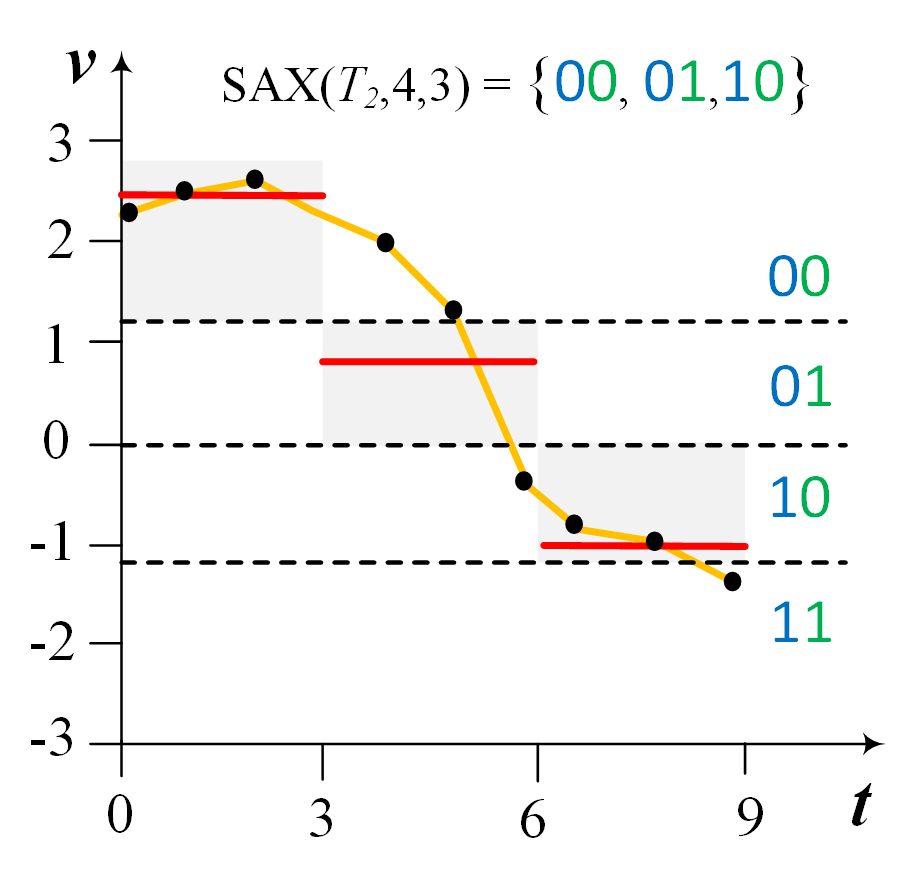
\includegraphics[width=0.23\textwidth]{figures/sax2.png}\label{subfig:isax_representation}}
 \subfloat[MBTS for two sets of time series]{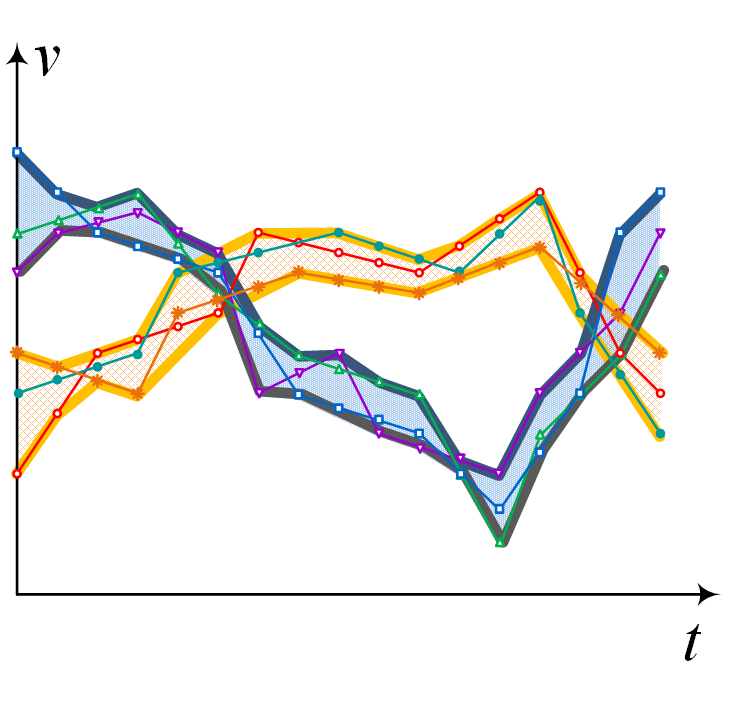
\includegraphics[width=0.23\textwidth]{figures/bounds_ctsr.png}\label{fig:example_bundle}}
\caption{SAX and MBTS representations over time series.}
\label{fig:isax_example}
\end{figure}


%%%%%%%%%%%%%%%%%%%%
\eat{
SAX representation of the time series shown in the example using w=3 words and cardinality 4:
SAX(T1, 4, 3) = { 00, 01, 11}
SAX(T2, 4, 3) = { 00, 01, 10}
SAX(T3, 4, 3) = { 00, 01, 01}
SAX(T4, 4, 3) = { 10, 01, 01}
SAX(T5, 4, 3) = { 01, 00, 00}
SAX(T6, 4, 3) = { 00, 10, 01}
SAX(T7, 4, 3) = { 01, 00, 00}
SAX(T8, 4, 3) = { 01, 10, 10}
}
%%%%%%%%%%%%%%%%%%%%%



\subsubsection{The \isax Family of Indices}
\label{subsec:isax}

Consider the dataset shown in Figure~\ref{subfig:sample}. By completely ignoring the spatial locations and using the SAX representations of all time series in this dataset, an \isax index \cite{shieh2008kdd} can be built as illustrated in Figure~\ref{subfig:isaxtree}. The root node captures the complete \isax space. It does not contain any SAX words, it only points to its children nodes (in the worst case, their number is $2w$). Each leaf has a pointer to a disk file containing the raw time series that it represents. The leaf itself also stores the \isax word of highest cardinality among these time series. An internal node designates a split in SAX space and is created when the number of time series contained by a leaf node exceeds a fixed capacity $M$. This split is binary and is made at a given position $j=1..w$ of the SAX word using a round-robin policy, so it always yields two children that differ on their $j$-th symbol while replicating the rest from their parent node. In essence, the SAX space represented by every node fully contains the union of the SAX spaces of its subtree.

Searching for time series similar to a query $q$ simply traverses the \isax tree, looking for a leaf node having the same \isax word as query $q$. The respective raw time series are fetched from disk and a sequential scan identifies those matching with $q$. 

%Improvements over the original \isax basically alleviate the bottleneck of expensive I/O when building the index for large datasets; our methodology in Section~\ref{subsec:isax_appr} is based on the latest $i$SAX2+ \cite{camerra2014kais}.




\begin{figure}[!t]
 \centering
\begin{minipage}[!t]{0.59\linewidth}
 \subfloat[Sample dataset with MBRs over objects]{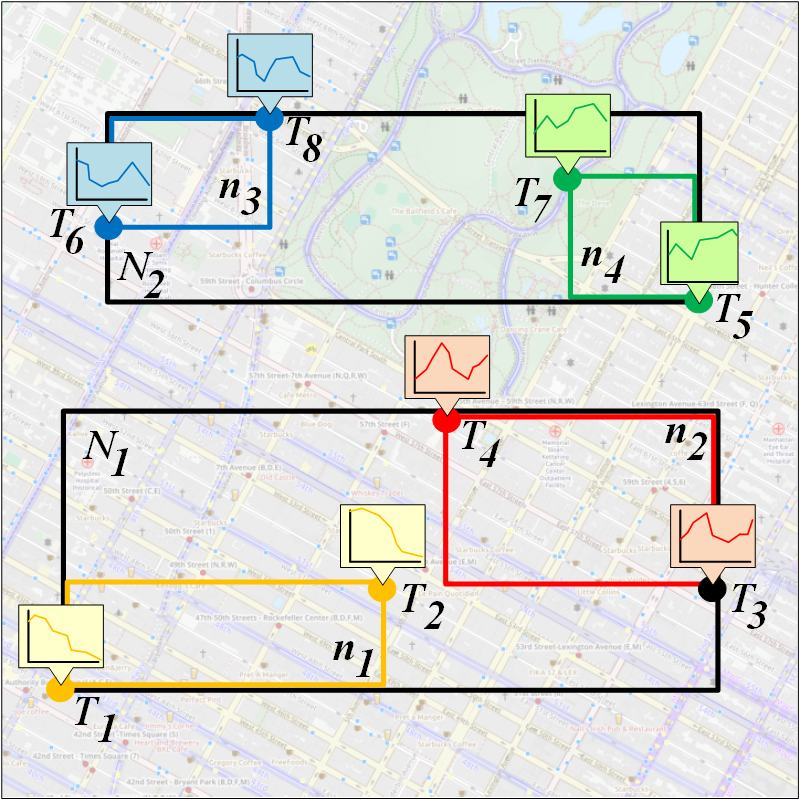
\includegraphics[width=50mm]{figures/geotimeseries.png}\label{subfig:sample}}
 \end{minipage}
\begin{minipage}[!t]{0.4\linewidth}
\subfloat[Spatial-only R-tree index]{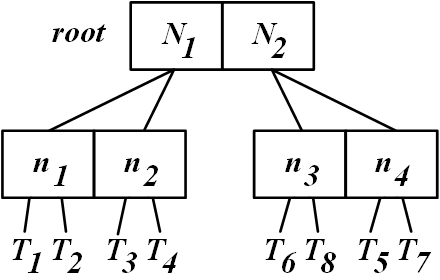
\includegraphics[width=36mm]{figures/r_tree.png}\label{subfig:rtree}}
\subfloat[Hybrid \btsr index]{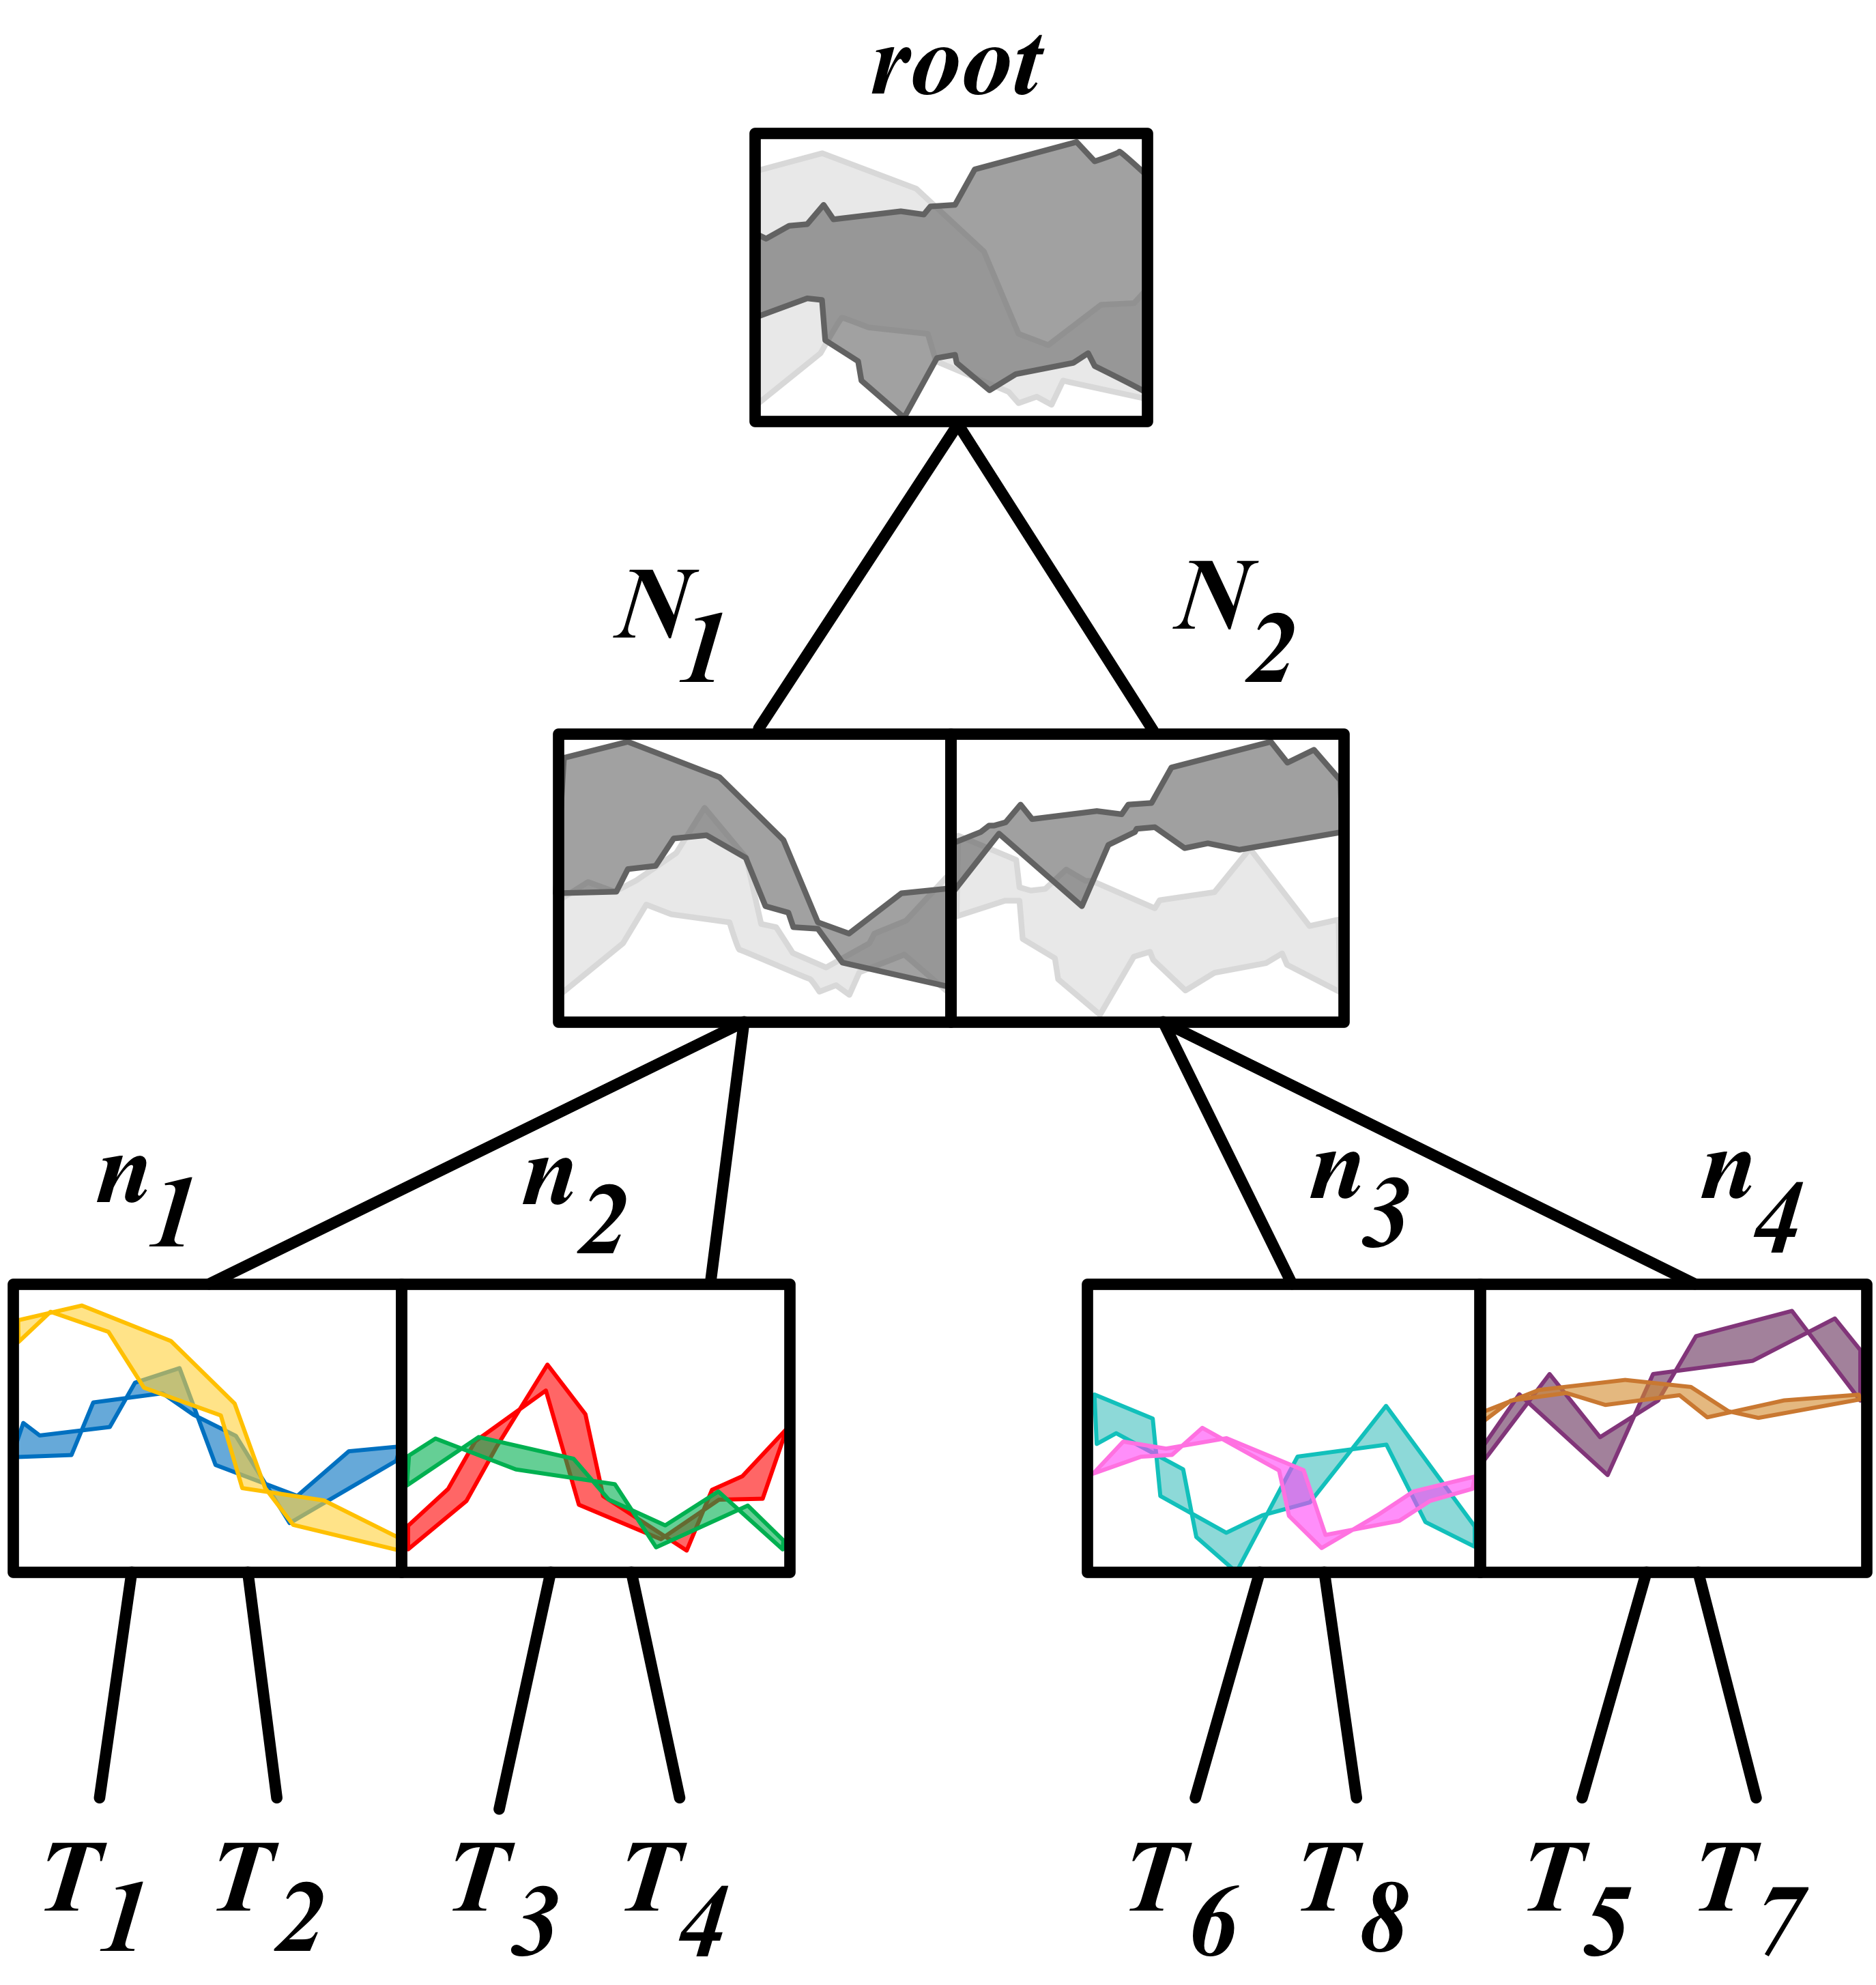
\includegraphics[width=36mm]{figures/btsr_tree.png}\label{subfig:btsrtree}}
\end{minipage}
\subfloat[\isax index over time series only (subtrees under dash lines not shown)]{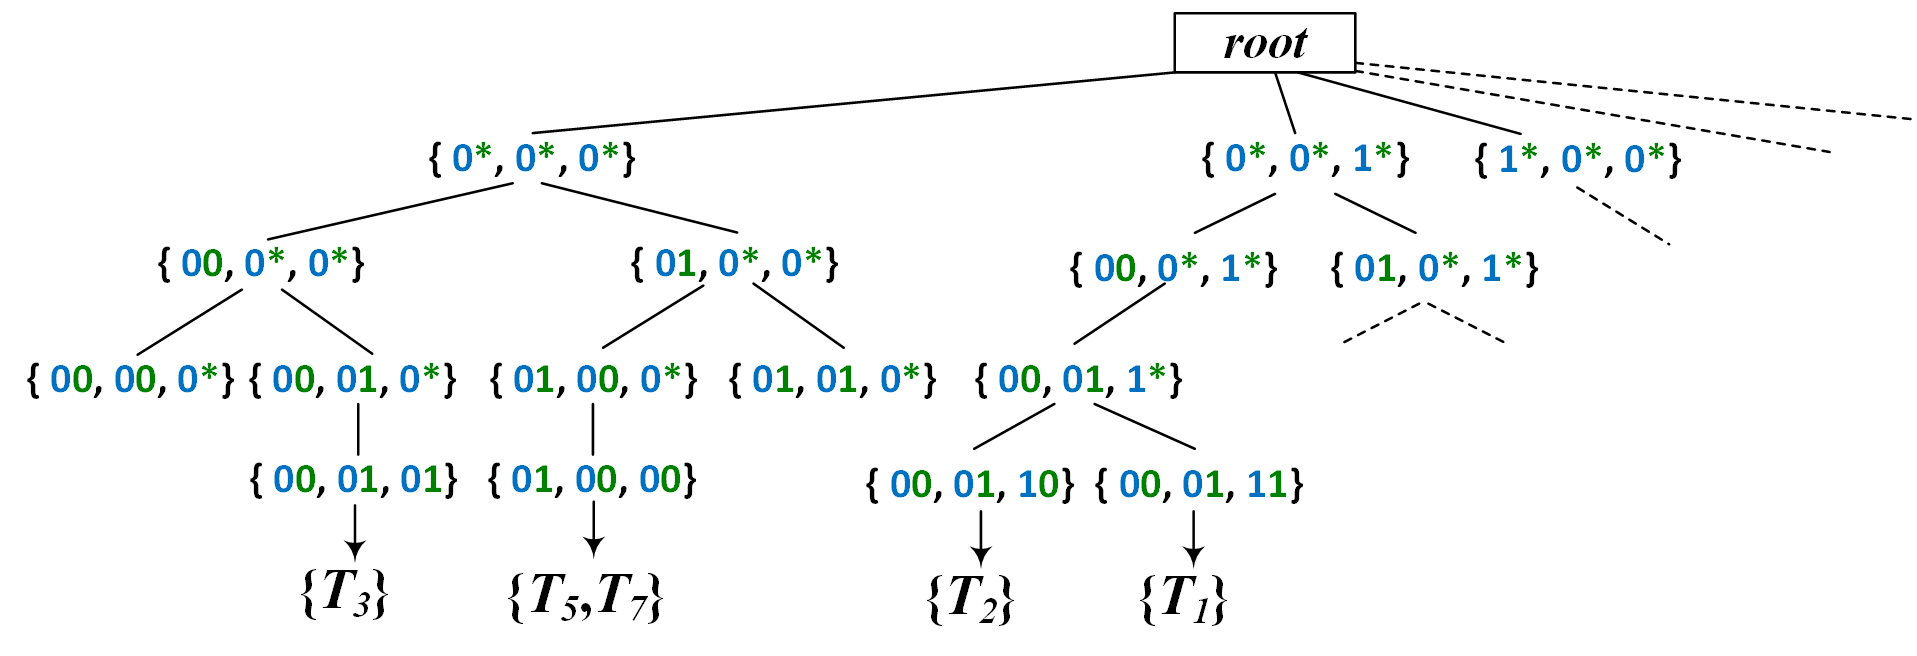
\includegraphics[width=0.49\textwidth]{figures/isax_tree2.png}\label{subfig:isaxtree}}
\caption{Indexing schemes over geolocated time series.}
\label{fig:example}
\end{figure}



\subsubsection{Minimum Bounding Time Series}
\label{subsec:mbts}

In \cite{chatzig17btsr}, we introduced the notion of {\em Minimum Bounding Time Series} (MBTS), which abstracts {\em a set of time series}  $\mathcal{T}$ using a pair of bounds that fully contain all of them.  Figure~\ref{fig:example_bundle} depicts an example of two MBTSs for two disjoint sets of time series. Formally, given a set of time series $\mathcal{T}$, its MBTS consists of an \emph{upper bounding time series} $B^{\sqcap}$ and a \emph{lower bounding time series} $B^{\sqcup}$, constructed by respectively selecting the maximum and minimum of values at each time point $i \in \{ 1, \dots, n \}$ among all time series in set $\mathcal{T}$ as follows:
\begin{align}\label{eq:bounds1}
 \begin{split}
  & B^{\sqcap} = \{ \max_{T \in \mathcal{T}} T.v_1, \ldots, \max_{T \in \mathcal{T}} T.v_{n} \} \\
  & B^{\sqcup} = \{ \min_{T \in \mathcal{T}} T.v_1, \ldots, \min_{T \in \mathcal{T}} T.v_{n} \}
 \end{split}
\end{align}

Note that both bounding time series have the same length $n$ as those enclosed within this MBTS.


\subsubsection{The \btsr Index}
\label{subsec:btsr}

A \btsr is constructed exactly as an R-tree \cite{Guttman1984} with respect to the spatial contents of a geolocated time series dataset, as depicted in the example of Figure~\ref{fig:example}. However, besides MBRs, nodes also store MBTSs, shown as colored strips per node in Figure~\ref{subfig:btsrtree}. Thus, the search space can be efficiently pruned when evaluating hybrid queries combining time series similarity with spatial proximity.

\eat{
The R-tree organizes a hierarchy of nested $d$-dimensional rectangles. Each node corresponds to a disk page and represents the MBR of its children or, for leaf nodes, the MBR of its contained geometries. The number of entries per node (excluding the root) is between a lower bound $m$ and a maximum capacity $M$. Query execution in R-trees starts from the root. MBRs in any visited node are tested for intersection against the search region. Qualifying entries are recursively visited until the leaf level or until no further overlaps are found. Several paths may be probed, as multiple sibling entries could overlap with the search region. 
}

As in R-trees, each node of the \btsr has at least $m$ and at most $M$ entries and stores the MBRs of its children. Additionally, for each child, a node stores a pre-specified number of MBTSs, each one enclosing all the time series indexed in its subtree. Each MBTS is calculated according to Eq.~\ref{eq:bounds1}. Construction and maintenance of the \btsr follow the procedures of the R-tree for data insertion, deletion and node splitting. Objects (i.e., geolocated time series) are inserted into leaf nodes and any resulting changes are propagated upwards. Once the nodes have been populated, the MBTS of each node are calculated bottom-up, relying on $k$-{\em means clustering} according to their Euclidean distance in the time series domain. The example in Figure \ref{fig:example_bundle} depicts the $k=2$ MBTSs (as two bands with a thick outline) obtained for a set of time series (shown as thin polylines). In a \btsr, each parent node receives all the MBTSs of its children and computes its own $k$ MBTSs. The process continues upwards, until reaching the root. 

%\checknote{{\bf Suppress for brevity?} Optionally, \emph{Piecewise Aggregate Approximation} \cite{keogh2001paa,faloutsos2000vldb} can be applied over the time series. As detailed in \cite{chatzig17btsr}, this allows a trade off between the number of clusters per node and the MBTS resolution, thus permitting a larger number ($>k$) of clusters in nodes at higher levels in the tree hierarchy.}